\documentclass{article}

\usepackage[final,nonatbib]{nips_2017}

\usepackage[utf8]{inputenc} % allow utf-8 input
\usepackage[T1]{fontenc}    % use 8-bit T1 fonts
\usepackage{hyperref}       % hyperlinks
\usepackage{url}            % simple URL typesetting
\usepackage{booktabs}       % professional-quality tables
\usepackage{amsfonts}       % blackboard math symbols
\usepackage{nicefrac}       % compact symbols for 1/2, etc.
\usepackage{microtype}      % microtypography

\usepackage[backend=biber]{biblatex}
\addbibresource{re-reika.bib}

\usepackage{graphicx}
\graphicspath{ {images/} }

% https://tex.stackexchange.com/questions/376420/include-chinese-characters-into-article-in-xelatex
\usepackage{fontspec}
\newfontfamily\cjkfont{Noto Sans CJK SC}

\usepackage{listings}

\title{Re-Reika: Engineering a DSL compiler}

\author{
Pinglei Guo \\
\texttt{piguo@ucsc.edu}
}

\begin{document}

\maketitle

\begin{abstract}
    We redesigned our DSL for time series database Reika to be more general purpose.
    It's statically typed without type inference,
    eager runtime check is added to ensure type of external data source.
    Its compiler is divided into multi phases and use immutable AST for parallel and incremental compilation.
    A working small language \verb+SimpleBin+ is provided while the real implementation is under heavy construction.
\end{abstract}

\section{Introduction}
\label{sec:introduction}

\subsection{Motivation and Accomplishment}
\label{subsec:motivation}

We decided to continue the development of Reika \footnote{\url{https://github.com/xephonhq/tsdb-proxy-java/tree/master/ql}},
a DSL for time series database previously built in CMPS203.
\footnote{\href{https://github.com/xephonhq/tsdb-proxy-java/blob/master/ql/Reika\_TSDB\_DSL\_0.0.1.pdf}{Reika\_TSDB\_DSL\_0.0.1.pdf}}.
However, in this quarter, we mainly focused on more detailed design (type system etc.)
and how to make the compiler extensible and maintainable.
Also we no longer limit it to time series data, we want it to be able to handle common data analytic tasks, even simple machine learning.

Due to the duration of the quarter, half of the time was spending on survey and building small prototype.
A survey of q, juila, kotlin, groovy, scala, dotty, weld~\cite{palkar2017weld}'s design and compiler implementation is listed in \verb+doc/dev-notes/at15+.
We implemented simply typed lambda calculus (\verb+simplebool+) and preceding exercises from TAPL in Java.
\footnote{located in tapl folder}
A typecheker, interpreter and transpiler for \verb+SimpleBin+ (only has int and boolean) \footnote{located in playground package of Reika}
to demonstrate how our real implementation is structured and the relation ship between typechecker, interpreter and transpiler.
The real Reika implementation is written from scratch without using old Reika codebase,
and because of a major refactor in the middle \footnote{\url{https://github.com/at15/reika/pull/31}} due to design flaw in AST and compiler phases, the latest version is currently stuck on
\verb+namer+ (symbol and scope) and \verb+typechecker+ phases,
it will be continued and integrate into author's master thesis during winter break and final quarter.

\subsection{Why Reika DSL instead of Python or SQL}
\label{subsec:why-reika}

A common question asked by friends of mine is why don't you just use python,
which is widely used in big data and machine learning as glue language.
The reason is python is not statically typed and it has a lot of legacy,
even though 3.6 adds type hint, most libraries don't have it, not to mention those struggle between python2 and python3.
When you run a python program,
it can execute 999 lines but throw error at last line because you concat a int to string when you try to save the result.

Languages like SQL is typed, but it is checked against schema until it is sent to server,
we want error when I typed invalid column name in editor.
Also there is always a layer of conversion between SQL query result and the code you used to implement bossiness logic
like generating report and graph, extra check is needed everywhere, they should be unified.

We want a language for data analytic that fails fast, has good editor integration.
It should be interactive for exploration and have good performance when run in production.
Which leads to our statically typed, mostly declarative DSL - Reika.
The rest of the paper is organized as following,
Section~\ref{sec:design} describes current syntax and semantic,
the choice we made in our type system and the overview of the compiler structure.
Section~\ref{sec:implementation} shows the progress so far and specific problems we have solved.
Section~\ref{sec:related-work} list related work and our difference with them.
Section~\ref{sec:future-work} contains the priority of unfinished work and potential new features.
Section~\ref{sec:conclusion} concludes the paper.

\section{Design}
\label{sec:design}

\subsection{Syntax}
\label{subsec:syntax}

The new syntax of Reika is mainly modeled after Q\footnote{http://code.kx.com/q/},
and syntax from Java-like language to make it easier to learn and maintain.
In Q, list and record are basic data structure, the underlying database can be represented as (flip of) a record of list,
how the data is actual stored on disk and memory is hidden to the user\footnote{Q is not open source}.
We do not use indent to structure code, because it makes parser and auto format easier to implement.
\footnote{We are using parser generator ANLTR, which is already pretty easy, but there is no harm to reduce complexity}
Semicolon is used to split expressions and curly brackets are used to group expression together for function and control blocks.

% FIXME: there is no ident for function
\texttt{/* \\
@author: at15 \\
@time: 2017-12-15 \\
*/ \\
val x:Int = 1; \\
val y:List[Int] = x + [1, 2, 3]; // [2, 3, 4]:List[Int] \\
plot([1,2,3], y) // a graph shows in browser \\
func a(x:Int, y:Int): Int \{ x + y; \} \\
val z = a(x, 2); // 3:Int \\
\\
val months = [1:5]; // [1, 2, 3, 4, 5] \\
val incomes = 5 rand\_from [10, 25]; // [10, 25, 25, 10, 10] \\
val account\_book = make\_table(\{ months: months, incomes: incomes \}); \\
print(account\_book); \\
| months | incomes | \\
|   1    |   10    | \\
|   2    |   25    | \\
val m = select max(incomes) from account\_book; // 25:Int\\
val ms = select months, incomes from account\_book where incomes > 10; // {months: [2. 3], incomes: [25, 25]} \\
val ms2 = ms.incomes + m // {months: [2. 3], incomes: [50, 50]} \\
\\
val stock: \{tm: List[Date], price: List[Float], symbol: List[String]\} = read\_csv("2016-Jan-01-stocks.csv") \\
% TODO: https://stackoverflow.com/questions/7745609/sql-select-only-rows-with-max-value-on-a-column
val company = select symbol from stock where price is max(price); // AAPL:String
}

Above shows the syntax of new Reika (from design spec, the implementation is not ready).
As you may noticed, type can be omitted in several places except function parameters, and variables are not mutable.
Add operator can broadcast (is overloaded) \texttt{1 + [1, 1]} is interpreted as \texttt{[1, 1] + [1, 1]}.
SQLish query can be executed directly on record of list after it is converted to table,
and data can be read from file or other data source, validation and conversion is performed by the runtime.

\subsection{Type System}
\label{subsec:type-system}

\subsubsection{No Type Inference}
\label{subsubsec:no-type-inference}

As a statically typed language, we chose to explict specify type instead of using inference.
The main reason is we want to support overloading (ad-hoc polymorphism),
so we can write \texttt{1 + [1, 2, 3]} instead of \texttt{1 +l [1, 2, 3]}.
This is more like a syntax sugar because it is resolved at compile time for performance.
However, it's hard to do type inference when overloading is involved (same syntax structure can result in multiple constraints),
the type system in Reika is quite limited, so we chose overload over type inference.

However, even without type inference, type specification can be omitted in certain places,
variable don't need to explict specify type (i.e. \verb+val x = 1+ instead of \verb+val x:Int = 1+)
because it can be computed from right hand side (like C++'s new \verb+auto+ keyword).
This is \textbf{not} type inference in ML languages like OCaml, Haskell.
The difference between compute type and inference type has confused me a lot (before taking the course).
From implementation side, compute type just need one pass, while inference need two pass, one for generating constraint, one for solve it (unification).
Considering the following lambda calculus (sort of) example:

\begin{center}
    ($\lambda$ x. y = x + 1) and ($\lambda$ x:Int. y = x + 1)
\end{center}

The first one need type inference for y while the second one just compute the type
because the first one has variable \verb+x+ with unbounded type.
The only way to introduce variable (w/ or w/o type) is using function (declaring variable in global space can be think
as the entire program is a function), as long as the function parameter has type, you don't need type inference, you just
simply compute the type because there won't be variable with unbounded type on 'rhs'.
\footnote{TODO: it should be proved, could be wrong, but a quarter is too short for making things sound}

But we still suggest user putting type even when it not necessary needed, because it serves as documentation,
if you write \verb+val x =+ and went for a coffee, you might not remember what you were trying to do 5 mins ago,
but if you write \verb+val x:Int =+, it is a cache that limit the search domain in your head.
This also applies to large projects as well, it is much better than writing a comment \verb+/* x is int*/ val x = 1.0+.
Documentation can't keep up with the rapid iteration, but compiler can, it will throw error you if you write \verb+val x:Int = 1.0+.

\subsubsection{Type check with external data source}
\label{subsubsec:type-check-with-extrenal-data-source}

Since one of our motivation is to fail early, all operation related with external data source such as file, database
are paid extra attention.
Before running the actual code, the runtime would try to valid all the data source are available and has the right type
\footnote{TODO: there should be formal name and existing implementation in literature, but I didn't find any so far},
i.e. a csv file should exists, and can contains more column but not less (subtype),
and the type should match what the user specified.
Normally, user have to implement those guardian code in languages like python, and a lot of time I find it verbose and repetitive.
So we decide to put it into the language.
However, we don't allow pass type to function, so it should be a hack in compiler implementation,
where data source related built in function need to look at the left hand side for expected type.
The reverse of this (kind of) is known as information based programming in F\# \footnote{http://thorium.github.io/FSharpAzure/2-DataUsage/DataUsageEng.html}.
It might be possible to do similar in Reika, with syntax like \texttt{type Stock = load\_type\_from\_csv("2016-Jan-01-stocks.csv")},
those two does not has conflict, one is eager runtime check, another is type system aided by data source at compile (develop) time
(the data source must be reachable when compile).

\subsection{Compiler Architecture}
\label{subsec:compiler-architecture}

Previous design and implementation of Reika targets query language like SQL, making its compiler simple.
Symbol and type checking are put into single traverse when constructing AST from parse tree.
The interpreter then execute AST to get the result, there is no user defined function and variable is mutable.
And since user can't define function, everything is implemented in host language and provided as builtin,
the is not concept like package or module.
However, since we want to make Reika more general, the old design is too restrictive.

\begin{center}
  \verb+REPL/file+ > \verb+ANTLR(lexer&Parser)+ > \verb+Symbol&Type(AST)+ > \verb+Interpreter+
\end{center}

The new design of Reika allow user to define function, and part of standard library is written in Reika,
reduce the burden of the host language when porting.
And this forces us to split symbol and type checking from constructing AST and do it in multiple phases.

\begin{figure}[h]
    \centering
    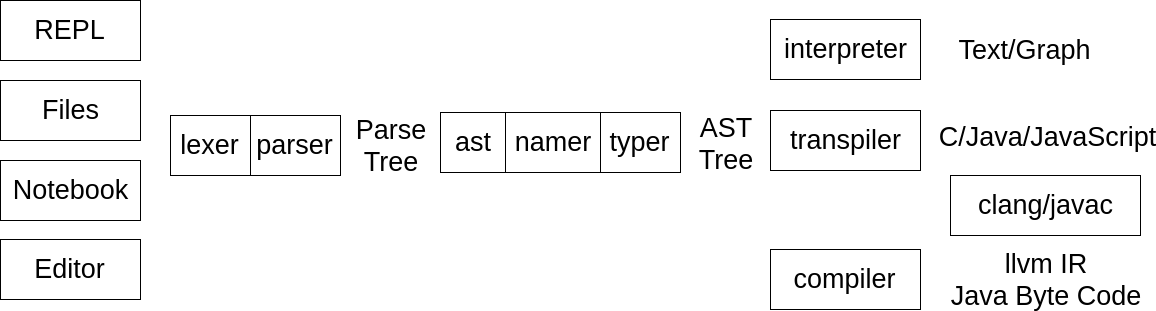
\includegraphics[width=\columnwidth]{reika-compiler}
    \caption{New Reika Compiler design}
    \label{fig:reika-compiler}
\end{figure}

As shown in figure~\ref{fig:reika-compiler}, its input can also be notebook or editor,
so it should be able to start a compiler server and do compile incrementally,
also using a compiler server increase compile speed even without incremental compile when we wrote compiler in language with JIT like Java.
Extra phase (\verb+ast+) after parser is needed because we only get a Parse Tree after using ANLTR, and we need a cleaner AST.
The typed AST can go three directions (in parallel).
For interpreter, it gives back text and graph directly.
For transpiler, based on code template, the AST is converted to C/Java/JavaScript,
target language need to have standard library implemented, external compiler is called to compile the generated code.
For compiler, we can generate LLVM IR or Java Byte Code directly, skipping the call to external compiler,
though since it's hard to do the optimization right, it might be better to sacrifice compile time for correctness and runtime performance.

% TODO: multi dialect
% TODO: unify compiler, interpreter, transpiler
% TODO: 伪编译语言算不算编译语言? - 梨梨喵的回答 - 知乎
% https://www.zhihu.com/question/263559593/answer/270924481
% 二村射影 https://en.wikipedia.org/wiki/Partial_evaluation

\section{Implementation}
\label{sec:implementation}

As a lesson from previous Reika, new Reika implementation is broken into several stages.
First we wrote implementation of TAPL assignment in Java \footnote{\url{https://github.com/at15/reika/tree/master/tapl}}, we compared with the reference OCaml implementation
to make sure the output is consistent, the parser is generated using ANLR as usual.
A small language with only Nat and Bool called \verb+SimpleBin+
\footnote{\url{https://github.com/at15/reika/tree/master/impl/reika-j/src/main/java/me/at15/reika/playground}}
was then created to play with visitor pattern,
and the relationship between typechecker, interpreter, transpiler.
A sample output is in Appendix figure~\ref{fig:simplebin}.

The main gain from implementing \verb+SimpleBin+ is interpreter, typechecker, transpiler all use AST,
they just operate on different abstraction level.
For a literal 1, a interpreter sees an integer 1,
a typchecker sees a term with type int, it is 1 or 100 does not matter,
a transpiler to C sees \verb+printf("\%d", 1)+,
a compiler to machine code sees \verb+MOV EAX, 1h+.
They all rely on the shape of the tree (syntactic form) to use rules,
and update certain state when ascending and descending trees (symbol table etc.).
Even lexer and parser are similar to them in some sense, instead of traversing trees,
lexer go through characters and parser go through tokens generated by lexer and yield trees.

The compiler implementation largely inspired by Scala and the new Dotty compiler in some aspects.
It is divided into multi phases as shown in figure~\ref{fig:reika-compiler}.
Some phases are parallel (i.e. transpile to C and Java), while some relies on another (i.e. \verb+ast+ after \verb+parser+).
Each phase has \verb+runsAfter+ attribute,
and the total phases are assembled by computing a DAG of phases when the compiler starts.
Hard code phases may give us more hint in development and better performance,
but we want compiler plugin in the future like \verb+scalc+,
allowing user inject a plugin to do things like changing all the positive number to negative number.

\verb+Phase+ just implement a simple interface \verb+void run(CompilationUnit unit)+,
errors are recorded instead throwing exception because we want to capture as much error as possible until we really can't move on.
This allow user to be more productive.
Each file is wrapped in a \verb+CompilationUnit+, which contains parse tree, ASTs and reference to file/string.
AST is immutable, traversing AST always create new AST instead of update in place,
so parallel access to the AST should not cause subtle bugs,
this may cause memory usage issue of compiler in the future when we have a larger standard library in Reika.

We are trying to mimic the new Denotation design in Dotty.
In dotty, compilation can be seen as a series event in time,
code can have different type in different run and phases.
i.e. When a external module is reloaded, compiled code relying on that module may no longer hold.
It's main use case is for incremental compile in large codebase.
We want a similar design because in a REPL environment,
it is incremental compile, you never know what the user gonna enter and we like REPL a lot.
Also storing trees at different Period
(in Dotty, runId and phaseId construct a period, symbol and scope are also associated with Denotation,
you obtain Denotation by giving Period and Tree) is useful for debugging the compiler,
user can travel back in time to see what was happening to the AST.
For performance, they use copy on write, for simplicity, we just deep copy everything and increase jvm memory.

Since the real Reika compiler is relatively complex, there is no end to end running code for now.
\verb+irk+ and \verb+reikac+ can only show help, most running example is in unit test.
Also we did a major refactor in the middle after survey on Scala and Dotty,
so working code for namer and typer are removed in PR\#31 \footnote{\url{https://github.com/at15/reika/pull/31}},
and we are still (re)implementing namer and typer,
work for standard library relies on what we want to do with package (module), and we are still finding
a middle ground because we want to transpile it to different languages, which all have different mechanism for module.

\section{Related Work}
\label{sec:related-work}

Weld~\cite{palkar2017weld} is an IR implemented in Rust for BigData,
it's aim is to use its syntax to force user write in a way that compiler can optimize the code to make use of parallel hardware.
We'd like to apply its optimization phase in Reika, which currently has none (\texttt{1 + 1} is still \texttt{1 + 1} after compile in Reika).
One of its core features is seamless integration with existing frameworks like Pandas, Spark etc.
But we don't want that, wide adoption means dealing with legacy and comparability issues.
Reika should be a small language for boosting productivity.

Q is Kx system's proprietary language for their time series database,
latter is used by many financial companies for analysing stock.
It's syntax requires a lot training for programmer with C-like background,
and the error message is too abbreviate to be used with editor.
It is dynamically typed so it can fail in the middle, and only experienced Q programmer can figure out the location based on the message.
We want to Reika to be a open source alternative to similar tasks and
put it into our own time series database (Xephon-K\footnote{\url{https://github.com/xephonhq/xephon-k}})

Dotty is the new Scala compiler, and will become Scala 3.0 in the future,
its type system has improved (LightBend used to be called TypeSafe after all).
And using denotation in compiler is a major change.
We want to mimic its compiler design,
but we don't want a complex type system, we just want to sit in the low corner of lambda cube.

Rezoom.SQL\footnote{\url{https://github.com/rspeele/Rezoom.SQL}}
\textit{typechecks a common SQL dialect and translates it to various RDMS backends} is implemented in F\#.
The first idea we have for Reika's type system is to type the data source so developer can have better autocomplete, and Rezoom.SQL is pretty close to that.
It is sad considering F\# has many cool features and is still not very popular, C\# shares similar fate.
%so we should not expect Reika to have more than one user.

\section{Future Work}
\label{sec:future-work}

Most future work should be implementing the design and try not to over engineer and pre-optimize.
It could become a playground for implementing various language features and used as a teaching resource.
It would be good to have its type system proved in Coq.

Editor plugin for VSCode and Intellij is needed.
VSCode has a language server protocol, which is vendor independent.
Intellij is powerful, but seems require everything to be implemented in their own framework.

We also want to add dialect to it, so certain features can be switched on/off based on dialect,
i.e. a Reika file without any IO call can be used as a typed configuration file.

It is also interesting if we could use Reika to describe a distributed system, similar works has been
done in unison\footnote{\url{https://github.com/unisonweb/unison}}.
Making a compiler for distributed system is interesting
when there are already many 'kernel' for distributed system like Mesos, Kubernetes.

Also since everything is related with machine learning these days, there are many DSL for machine learning rising,
though none have shaken the ground for python.
It would be good if we can put machine learning into Reika's standard library and squish it into our time series database,
it is often considered a bad practice to couple storage and compute, but hardware is changing,
data is becoming larger, it might be cheaper to move computing to data instead of vice verse.

\section{Conclusion}
\label{sec:conclusion}

We redesigned Reika and its compiler to make a more general DSL.
It's implementation is still in early stage.
We are expecting to integrate it into our time series database next (also last) quarter.

The authors would like to thank his presentation buddies Tien and Alif.
Chujiao's contribution on previous version of Reika also helps shaping the new version.

The code for Reika can be found on GitHub \href{https://github.com/at15/reika}{at15/reika}.

\printbibliography

\section*{Appendix}
\label{sec:appendix}

\begin{figure}[h]
    \centering
    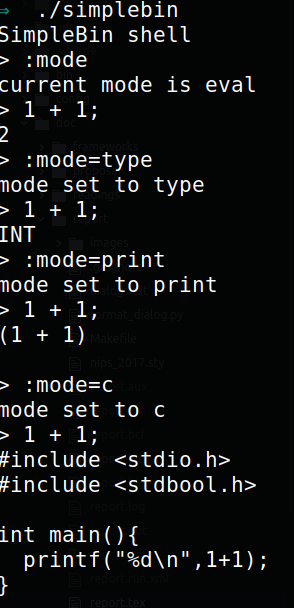
\includegraphics[width=0.5\columnwidth]{simplebin}
    \caption{SimpleBin interpreter, typechecker and transpiler}
    \label{fig:simplebin}
\end{figure}

\end{document}
